% BadmintonGRF @ ACM MM 2026 Dataset Track
% 基于 ACM 官方 acmart 模板（sigconf + screen；非匿名稿不加 review）

% !TEX root = badmintongrf-mm2026.tex
% Allow embedding vector figures exported as PDF 1.6+ (e.g. from SVG).
\pdfminorversion=7
% Enable \cellcolor in tables (acmart loads xcolor).
\PassOptionsToPackage{table}{xcolor}
\documentclass[sigconf,screen]{acmart}
% Allow line breaks inside \url/\path (paths, GitHub URLs) in two-column mode.
\usepackage{xurl}
\usepackage{dblfloatfix} % improves \texttt{figure*}/\texttt{table*} placement in \texttt{twocolumn} (fewer column holes)

%================ 投稿阶段建议设置 ================
% Dataset Track 一般为单盲：作者信息可见（不加 anonymous）
% 投稿阶段通常不需要填 DOI/ISBN；camera-ready 再按会议要求补全
\settopmatter{
  printacmref=true,
  printccs=true,
  printfolios=true
}

% 如官方要求去掉版权脚注，可打开下行（不同会议要求可能不同）
% \renewcommand\footnotetextcopyrightpermission[1]{}

%================ 宏包配置（数学 / 图表 / 参考文献辅助） ================
% acmart 已经加载：graphicx, xcolor, hyperref 等，避免重复
% 注意：acmart/newtxmath 与 amssymb 在部分 TeX Live 组合下会冲突（\Bbbk 重定义）
\usepackage{amsmath}            % 数学公式
\usepackage{booktabs}           % 表格的 \toprule, \midrule, \bottomrule
\usepackage{multirow}           % 表格多行合并
\usepackage{siunitx}            % 物理量与单位，\SI{1.23}{\newton\per\kilogram}
\usepackage[nameinlink,noabbrev]{cleveref} % 智能引用，\cref{fig:xxx,tab:yyy}
\usepackage{tabularx}           % 稳定两栏表格宽度
\usepackage{pifont}             % \cmark / \xmark in modality table
\usepackage{balance}            % even last-page two-column balance (ACM two-column body)
\usepackage{needspace}          % reserve space before \subsection to reduce orphaned half-columns
% Main text figures (replace placeholders when final art is exported):
%   Fig. 1 (teaser)    -> Introduction: multimodal task example (video/pose + GRF).
%   Fig. 2 (pipeline)  -> end of Related Work (before Sec.~3); avoids figure* + Sec.~3 column holes.
%   Fig. 3 (setup)     -> Section 3.1: instrumented court schematic.
%   Extra: LOSO scaling / camera plots -> supplementary website (6-page budget).
% Sync QC plots stay in the supplementary material.

\sisetup{
  detect-all,
  per-mode=symbol,
}

% Subtle de-emphasis styling for secondary table rows.
\newcommand{\muted}[1]{\textcolor{black!60}{#1}}
\newcommand{\cmark}{\ding{51}}
\newcommand{\xmark}{\ding{55}}

% Caption / float spacing: stay close to acmart defaults; avoid shrinking
% \abovecaptionskip too much (hurts caption readability). Fig.~2 must not
% reserve fixed height on \includegraphics (see Fig.~2 source) or a large
% empty band appears between the art and the caption.
\setlength{\abovecaptionskip}{6pt}
\setlength{\belowcaptionskip}{3pt}

% Tighter than the prior 14pt setting: top/bottom floats + following \subsection
% can stack (\textfloatsep + section heading glue) and read as ``3--4 blank lines''.
\setlength{\textfloatsep}{9pt plus 3pt minus 3pt}
\setlength{\floatsep}{10pt plus 4pt minus 2pt}
\setlength{\intextsep}{10pt plus 4pt minus 2pt}

% Bibliography in ACM proceedings is included in the PDF page count.
% We slightly increase bibliography item spacing to match the requested
% "6-page main text + 2-page references" layout.
\setlength{\bibsep}{0.32pt}

% acmart (sigconf) defaults to \flushbottom, which vertically stretches glue on
% short columns and can read as extra blank bands after headings and between
% short paragraphs; \raggedbottom keeps natural glue (column bottoms may be
% slightly ragged, which is typical for two-column proceedings).

%================ 论文元数据（标题与作者） ================
% Dataset track 的标题建议：短、直指“资源+可复现 benchmark”，避免像算法论文
\title{BadmintonGRF: A Multimodal Dataset and Benchmark for Markerless Ground Reaction Force Estimation in Badminton}

%================ Authors ================
% 说明：
% - 这里用拼音作为英文名（如需护照拼写/偏好写法可后续统一调整）
% - 单盲：作者信息可见
\author{Kuoye Niu}
\affiliation{
  \institution{School of Sports Engineering, Beijing Sport University}
  \city{Beijing}
  \country{China}
}
\affiliation{
  \institution{College of Control Science and Engineering, Zhejiang University}
  \city{Hangzhou}
  \country{China}
}
\email{kuoyeniu@163.com}

\author{Jianwei Li}
\affiliation{
  \institution{School of Sports Engineering, Beijing Sport University}
  \city{Beijing}
  \country{China}
}
\email{jianwei@bsu.edu.cn}

\author{Shengze Cai}
\affiliation{
  \institution{College of Control Science and Engineering, Zhejiang University}
  \city{Hangzhou}
  \country{China}
}
\email{shengze_cai@zju.edu.cn}


\author{Yong Ma}
\affiliation{
  \institution{Wuhan Sports University}
  \city{Wuhan}
  \country{China}
}
\email{mayong@whsu.edu.cn}

\author{Mengyao Jia}
\affiliation{
  \institution{Wuhan Sports University}
  \city{Wuhan}
  \country{China}
}
\email{2023420024@whsu.edu.cn}

\author{Lishun Shen}
\affiliation{
  \institution{Department of Physical Education, Zhejiang Gongshang University}
  \city{Hangzhou}
  \country{China}
}
\email{shenlishun@mail.zjgsu.edu.cn}

\author{Zhenheng Zhang}
\affiliation{
  \institution{Department of Sports Science, Zhejiang University}
  \city{Hangzhou}
  \country{China}
}
\email{zhzh@zju.edu.cn}

% \author{Yan Jiang}
% \affiliation{
%   \institution{Center for Medical Device Evaluation, National Medical Products Administration}
%   \city{Beijing}
%   \country{China}
% }
% \email{jiangyan@cmde.org.cn}

\author{Yuxin Peng}
\affiliation{
  \institution{Department of Sports Science, Zhejiang University}
  \city{Hangzhou}
  \country{China}
}
\email{pyxpeng@zju.edu.cn}


\author{Xian Song}
\authornote{Corresponding author.}
\affiliation{
  \institution{Department of Sports Science, Zhejiang University}
  \city{Hangzhou}
  \country{China}
}
\email{sx1993@zju.edu.cn}

% 关键词与 CCS 概念，按 ACM MM 要求填写
\begin{CCSXML}
<ccs2012>
   <concept>
       <concept_id>10010147.10010178</concept_id>
       <concept_desc>Computing methodologies~Computer vision</concept_desc>
       <concept_significance>500</concept_significance>
   </concept>
   <concept>
       <concept_id>10010405.10010444</concept_id>
       <concept_desc>Applied computing~Physical sciences and engineering</concept_desc>
       <concept_significance>500</concept_significance>
   </concept>
   <concept>
       <concept_id>10002951.10003227</concept_id>
       <concept_desc>Information systems~Multimedia databases</concept_desc>
       <concept_significance>300</concept_significance>
   </concept>
</ccs2012>
\end{CCSXML}

\ccsdesc[500]{Computing methodologies~Computer vision}
\ccsdesc[500]{Applied computing~Physical sciences and engineering}
\ccsdesc[300]{Information systems~Multimedia databases}

\keywords{dataset, multimodal learning, ground reaction force, badminton, biomechanics, sports video}

% --- compact typesetting helpers (avoid awkward line breaks) ---
\newcommand{\rateHz}[1]{\mbox{#1~Hz}}
% Public code/data URL.
\newcommand{\BadmintonGRFGitHubBase}{https://github.com/KenyaNiu/BadmintonGRF}
\newcommand{\BadmintonGRFRepo}{\url{\BadmintonGRFGitHubBase}}
\newcommand{\BadmintonGRFRepoShort}{\href{\BadmintonGRFGitHubBase}{project page}}
% Narrative pointer to extended tables/schema (files live in the GitHub tree; avoid in-paper paths).
\newcommand{\BadmintonGRFSupplementary}{\emph{Supplementary Material}}
% After the first spelled-out "quality assurance (QA)" in the abstract, use "QA" for short.
\newcommand{\QAabbrev}{QA}

%================ 正文开始 ================
\begin{document}
\raggedbottom

\begin{abstract}
Public multimodal resources rarely pair laboratory ground reaction force (GRF) with high-frame-rate multi-view video for \emph{non-periodic} court sports.
BadmintonGRF links eight-view \(\sim\)120\,FPS RGB, four Kistler plates, and Vicon C3D; without hardware genlock, software alignment uses human-verified events, automatic \emph{quality assurance} (\QAabbrev), and per-camera offsets with uncertainty metadata.
Tier~1 releases 2D pose and aligned GRF; Tier~2 provides raw RGB/C3D under application access.
We release 17{,}425 impact-segment archives (10-subject tree; 156 trials); after loader gates: 12{,}867 instances and 1{,}732 unique impacts (multi-view collapsed).
To our knowledge, no prior \emph{public} badminton resource combines this sensing stack with audited video--GRF alignment for impact-centric GRF estimation.
We open-source preprocessing, LOSO splits, ten baselines, and late fusion (single deterministic test forward pass, no TTA); a within-trial diagnostic is in \BadmintonGRFSupplementary.
Tier~1: CC BY-NC 4.0; Tier~2: privacy-controlled access.
\end{abstract}

\maketitle

%================ 1. Introduction ================
\section{Introduction}
Ground reaction forces (GRF) summarize external foot--ground loading and are closely tied to workload monitoring, fatigue accumulation, and lower-extremity injury risk \cite{lamBiomechanicsLowerLimb2020,pardiwalaBadmintonInjuriesElite2020,huCorrelationLowerLimb2022,valldecabresEffectMatchFatigue2022}.
Markerless estimates aligned to laboratory plates could eventually support the same monitoring goals in training halls---for example, workload-aware injury-risk screening and data-informed technical coaching---without requiring every session to be run on instrumented courts.
Accurate GRF measurement nonetheless relies on force plates and laboratory-grade synchrony (typically with marker-based motion capture), which is costly to deploy for continuous, unconstrained recording in routine training and competition \cite{evansSynchronisedVideoMotion2024,uhlrichOpenCapHumanMovement2023,werlingAddBiomechanicsDatasetCapturing2025}.
BadmintonGRF supplies \emph{study-grade} multimodal capture toward that gap: high-rate multi-view video, Vicon C3D kinematics, and ground-truth 6-axis GRF with software video--GRF alignment (consumer RGB is not genlocked to laboratory plates), human-verified event correspondences, and \QAabbrev{} review; the released LOSO benchmark emphasizes privacy-friendly pose inputs paired with aligned vertical \(F_z\) (Fig.~\ref{fig:overview}).

\begin{figure}[!t]
  \centering
  \includegraphics[width=0.98\linewidth]{figures/Fig1.png}%
  \caption{BadmintonGRF teaser. Top-to-bottom: motivation in impact-centric badminton movements, dataset resources with synchronized multi-view video/pose and laboratory sensing, and benchmark-ready GRF regression outputs. For each impact window, the model learns BW-normalized vertical force \((F_z)\) from visual cues with strict temporal alignment and protocol-aware metadata.}
  \label{fig:overview}
  \Description{Teaser figure of BadmintonGRF: an impact-centric learning setup with synchronized multi-view video and 2D pose streams aligned to laboratory vertical ground reaction force targets, plus benchmark outputs for GRF regression.}
\end{figure}

\paragraph{Why badminton and why now.}
Non-contact GRF estimation from video and pose has progressed \cite{mundt2022Estimating,ishida2024Estimation,hossain2025Knowledge}, but much of the evidence still comes from periodic locomotion or scripted jumps.
Competitive badminton is \emph{intermittent}: athletes change direction abruptly and land from jumps often, so foot--ground loading is less regular than in steady gait or rehearsed hop tasks.
Those movement demands are tied to match workload and lower-extremity stress in badminton-focused and sports-medicine studies \cite{lamBiomechanicsLowerLimb2020,pardiwalaBadmintonInjuriesElite2020,huCorrelationLowerLimb2022,tongEffectsAnkleDorsiflexor2023,valldecabresEffectMatchFatigue2022}.
Estimating GRF from vision or pose in this setting is therefore both harder (more irregular kinematics) and more representative of real court loading than benchmarks built mainly on stereotyped strides or single jumps.
Yet public resources rarely combine synchronized laboratory GRF, high-rate multi-view video, and a shared, reproducible benchmark for badminton impacts; that scarcity slows community progress on injury- and workload-aware monitoring and on comparable vision-to-GRF models for coaching-relevant feedback.
BadmintonGRF is built to close it by releasing plate-aligned multimodal captures, deterministic loaders, and fixed evaluation protocols.

\paragraph{Positioning vs. existing badminton datasets.}
FineBadminton focuses on fine-grained semantic understanding of badminton gameplay with hierarchical annotations and an MLLM-driven annotation pipeline \cite{heFineBadmintonMultiLevelDataset2025}.
BadmintonGRF instead targets \emph{biomechanical ground truth}: synchronized force-plate GRF and mocap for \emph{markerless} load estimation from video/pose, plus protocol-stratified metadata and a reproducible benchmark.
This division of scope motivates our Dataset Track framing: data quality, alignment fidelity, and reproducible evaluation are the central contributions.

\paragraph{Contributions.}
BadmintonGRF releases synchronized high-rate video, pose tracks, and laboratory GRF—modalities that align with the ACM Multimedia emphasis on multimodal content and sensor data. In line with Dataset Track expectations, the dataset and its evaluation protocols are the primary contributions; baselines are reproducible anchors rather than performance claims.
We contribute:
\begin{enumerate}
  \item \textbf{Study-grade multimodal capture for badminton impacts:} eight \(\sim\)120\,FPS RGB streams, four six-axis Kistler plates, Vicon C3D, and fatigue-stage protocol tags (Sec.~\ref{sec:dataset_stats}, Table~\ref{tab:stats}).
  \item \textbf{Reproducible preprocessing and alignment:} C3D-based GRF export, camera-wise video--GRF alignment, impact segmentation, and automatic synchronization \QAabbrev{} checks (Fig.~\ref{fig:pipeline}, Sec.~\ref{sec:sync_grf}).
  \item \textbf{Benchmark-ready released data:} 17{,}425 public segment archives for the 10-subject tree, with 12{,}867 retained instances after fixed quality gates and 1{,}732 unique impacts after multi-view collapse (Sec.~\ref{sec:dataset_stats}, Table~\ref{tab:stats}).
  \item \textbf{Reference benchmark suite:} fixed LOSO protocol, four core metrics, ten reproducible single-view baselines, optional late fusion, and a within-trial diagnostic with released scripts and fixed splits (Sec.~\ref{sec:experiments}, Table~\ref{tab:benchmark_all}, \BadmintonGRFSupplementary).
\end{enumerate}
Compared with model-centric studies, our emphasis is \emph{resource quality and reuse}: synchronized biomechanical ground truth, explicit alignment/\QAabbrev{} procedures, and deterministic benchmark loaders that reduce hidden implementation variance.

\paragraph{Relevance to ACM Multimedia.}
BadmintonGRF emphasizes three MM-relevant aspects: temporal alignment under heterogeneous clocks, tiered privacy-preserving release, and multi-view fusion under fixed protocols.
Tier~1 isolates temporal modeling from raw appearance.
Tier~2 enables RGB/C3D research under controlled access (Sec.~\ref{sec:benchmark_methods}).
We organize the paper as \emph{resource construction} (Sec.~\ref{sec:related}--Sec.~\ref{sec:dataset_stats}) followed by \emph{benchmark utility} (Sec.~\ref{sec:experiments}).

%================ 2. Related Work ================
\section{Related Work}
\label{sec:related}
We review prior badminton resources, synchronized biomechanics datasets, and pose-to-GRF modeling work, then position BadmintonGRF against their remaining gaps.
\subsection{Badminton Datasets and Understanding Benchmarks}
% Place Table~\ref{tab:modality_compare} immediately after the subsection heading so
% the float is less likely to sit above the 2.1 title with a large \textfloatsep gap.
\begin{table}[t]
  \centering
  \caption{Public resources: task focus, compact scale indicators, and bundled sensors. \textbf{MV}: multi-view video; \textbf{MC}: marker mocap; \textbf{GRF}: in-floor plates (\xmark{} = wearable-only pressure); \textbf{Ftg}: fatigue/protocol tags.}
  \label{tab:modality_compare}
  \footnotesize
  \begin{minipage}{\columnwidth}\sloppy
  \setlength{\tabcolsep}{2.1pt}
  \renewcommand{\arraystretch}{1.1}
  \begin{tabularx}{\columnwidth}{@{}>{\raggedright\arraybackslash}p{1.55cm} >{\raggedright\arraybackslash}X >{\raggedright\arraybackslash}p{1.45cm} cccc@{}}
    \toprule
    \textbf{Dataset} & \textbf{Focus} & \textbf{Scale} & \multicolumn{4}{c@{}}{\textbf{Sensing}} \\
    \cmidrule(l{2pt}r{2pt}){4-7}
     & & & \textbf{M} & \textbf{C} & \textbf{G} & \textbf{F} \\
    \midrule
    ShuttleNet~\cite{wangShuttleNetPositionAwareFusion2022} & Stroke forecasting; rally anticipation & 75 matches & \xmark & \xmark & \xmark & \xmark \\
    ShuttleSet~\cite{wangShuttleSetHumanAnnotatedStrokeLevel2023} & Singles stroke tactics & 44 matches & \xmark & \xmark & \xmark & \xmark \\
    \shortstack[l]{Fine\\Badminton}~\cite{heFineBadmintonMultiLevelDataset2025} & Hier.\ semantics; MLLM tasks & 120 matches & \xmark & \xmark & \xmark & \xmark \\
    \shortstack[l]{MultiSense\\Badminton}~\cite{seongMultiSenseBadmintonWearableSensor2024} & Wearable pressure \& perf. & 7{,}763 swings & \xmark & \xmark & \xmark & \xmark \\
    BioCV~\cite{evansSynchronisedVideoMotion2024} & Walk/run/CMJ/hop (lab) & 600 instr.\ trials & \cmark & \cmark & \cmark & \xmark \\
    \cmidrule[\heavyrulewidth](l{2pt}r{2pt}){1-7}
    \shortstack[l]{\textbf{Badminton}\\\textbf{GRF}} & \textbf{Impacts; GRF bench (LOSO)} & \shortstack[l]{\textbf{17,425} seg.;\\\textbf{1,732} uniq.$^{\dagger}$} & \cellcolor{black!4}\cmark & \cellcolor{black!4}\cmark & \cellcolor{black!4}\cmark & \cellcolor{black!4}\cmark \\
    \bottomrule
  \end{tabularx}
  \vspace{2pt}
  {\setlength{\baselineskip}{10pt}%
  \noindent\textbf{M}/\textbf{C}/\textbf{G}/\textbf{F} correspond to \textbf{MV}, \textbf{MC}, \textbf{GRF}, and \textbf{Ftg} in the caption.
  $^{\dagger}$On-disk impact windows / unique $(\text{trial},\text{impact})$ after quality gates (Sec.~\ref{sec:dataset_stats}).
  The public Tier~1 tree uses 10 subjects from 17 instrumented athletes.
  More rows: \BadmintonGRFSupplementary{}.}
  \end{minipage}
\end{table}
Prior badminton datasets emphasize tactics/semantics, not study-grade in-floor GRF + mocap at \(\sim\)120\,FPS multi-view video for landings \cite{wangShuttleSetHumanAnnotatedStrokeLevel2023,heFineBadmintonMultiLevelDataset2025,seongMultiSenseBadmintonWearableSensor2024}.
Table~\ref{tab:modality_compare} contrasts scale, focus, and sensing (\textbf{M}/\textbf{C}/\textbf{G}/\textbf{F}: MV/MC/GRF/fatigue tags).
ShuttleNet, ShuttleSet, and FineBadminton target rally understanding.
MultiSenseBadminton focuses on wearable sensing.
\textbf{BioCV} \cite{evansSynchronisedVideoMotion2024} is a laboratory multi-sensor resource, but not badminton-specific.
Extended multi-sport rows: \BadmintonGRFSupplementary{}.

\subsection{Multi-view Synchronized Biomechanics and GRF Estimation}
Multi-view settings improve observability under occlusion and viewpoint changes \cite{bragagnolo2025Multiview,cao2025KeypointNet}.
\textbf{BioCV} \cite{evansSynchronisedVideoMotion2024} is closest in sensing stack (multi-camera video, Vicon, force plates).
However, it targets \emph{stereotyped} locomotion in a gait-laboratory protocol and does not include badminton-specific court movements or fatigue-stratified trial tags.
\textbf{AddBiomechanics} \cite{werlingAddBiomechanicsDatasetCapturing2025} scales physics-driven modeling.
It does not provide our badminton-specific protocol, per-trial video--GRF offset review, or released impact-window benchmark.
BadmintonGRF fills this remaining gap with badminton-focused capture and an end-to-end alignment + impact-segmentation pipeline.

\subsection{From Pose/Video to GRF: Tracking and Temporal Modeling}
Learning-based non-contact GRF estimation from 2D video/pose is well studied \cite{ishida2024Estimation,mundt2022Estimating,hossain2025Knowledge,johnsonOnfieldPlayerWorkload2019,kim2025Estimation,gaoAutomatedRecognitionAsymmetric2023,bogaertPredictingVerticalGround2024}.
Modern pose/tracking backbones are also mature \cite{zhangByteTrackMultiobjectTracking2022,fangAlphaPoseWholeBodyRegional2023,linFeaturePyramidNetworks2017,linMicrosoftCOCOCommon2014,caoRealtimeMultiPerson2017,bazarevskyBlazePose2020,songHumanPoseEstimation2021,zhou2023Efficient,heDeepResidualLearning2016}.
What remains missing is a badminton benchmark with synchronized force-plate targets, unified quality filtering, and fixed LOSO evaluation.
BadmintonGRF addresses this gap with reproducible single- and multi-view baselines.

% Full-width Fig.~2 sits at the end of Sec.~2 (not inside Sec.~3 opening) so
% \texttt{figure*} does not interact with Sec.~3 headings; that pairing often
% yields a short first column with a large gap before the next \texttt{\textbackslash subsection}.
\begin{figure*}[!t]
  \centering
  % Width only: a fixed \texttt{height=} box with \texttt{keepaspectratio} leaves empty
  % vertical band under wide pipeline art and exaggerates the gap before the caption.
  \includegraphics[width=\textwidth]{figures/Fig2.png}%
  \caption{Released preprocessing flow: six left-to-right stages (A--F) from synchronized modalities through GRF extraction and alignment, pose and tracking, fixed-length impact segments, LOSO benchmark packaging with reference baselines and optional multi-view late fusion, and tiered public release; timing is handled continuously in seconds so mixed acquisition rates remain comparable. Court geometry is not shown (Fig.~\ref{fig:setup}).}
  \label{fig:pipeline}
  \Description{Six-stage horizontal pipeline (A--F): raw capture; GRF export and video--GRF alignment; pose and tracking; impact segments; LOSO benchmark with ten baselines and late fusion; tiered release.}
\end{figure*}

%================ 3. BadmintonGRF Dataset ================
\section{BadmintonGRF Dataset}
\noindent Figs.~\ref{fig:pipeline}--\ref{fig:setup} index stages A--F; subsections follow acquisition \(\rightarrow\) alignment \(\rightarrow\) segmentation \(\rightarrow\) release.

\subsection{Acquisition Setup}
BadmintonGRF was collected on an instrumented badminton court with \emph{co-located} multimodal sensing (Fig.~\ref{fig:setup}; Fig.~\ref{fig:pipeline}, Stage~A): up to 8 fixed RGB cameras (DJI Osmo Action 4, \(\sim\)120 FPS), 4 Kistler six-axis force plates, and 8-camera Vicon mocap (C3D). Inter-modal alignment uses per-camera human-annotated offsets (about one-frame precision) with automatic verification; Vicon and plates share a laboratory clock, while independently clocked RGB streams are aligned to GRF in software without hardware genlock (Sec.~\ref{sec:sync_grf}) \cite{evansSynchronisedVideoMotion2024,werlingAddBiomechanicsDatasetCapturing2025}. Optional IMU signals are excluded from the main LOSO benchmark due to calibration variability.

\begin{figure}[!t]
  \centering
  % Slightly narrower than column so the full-width pipeline figure remains visually primary.
  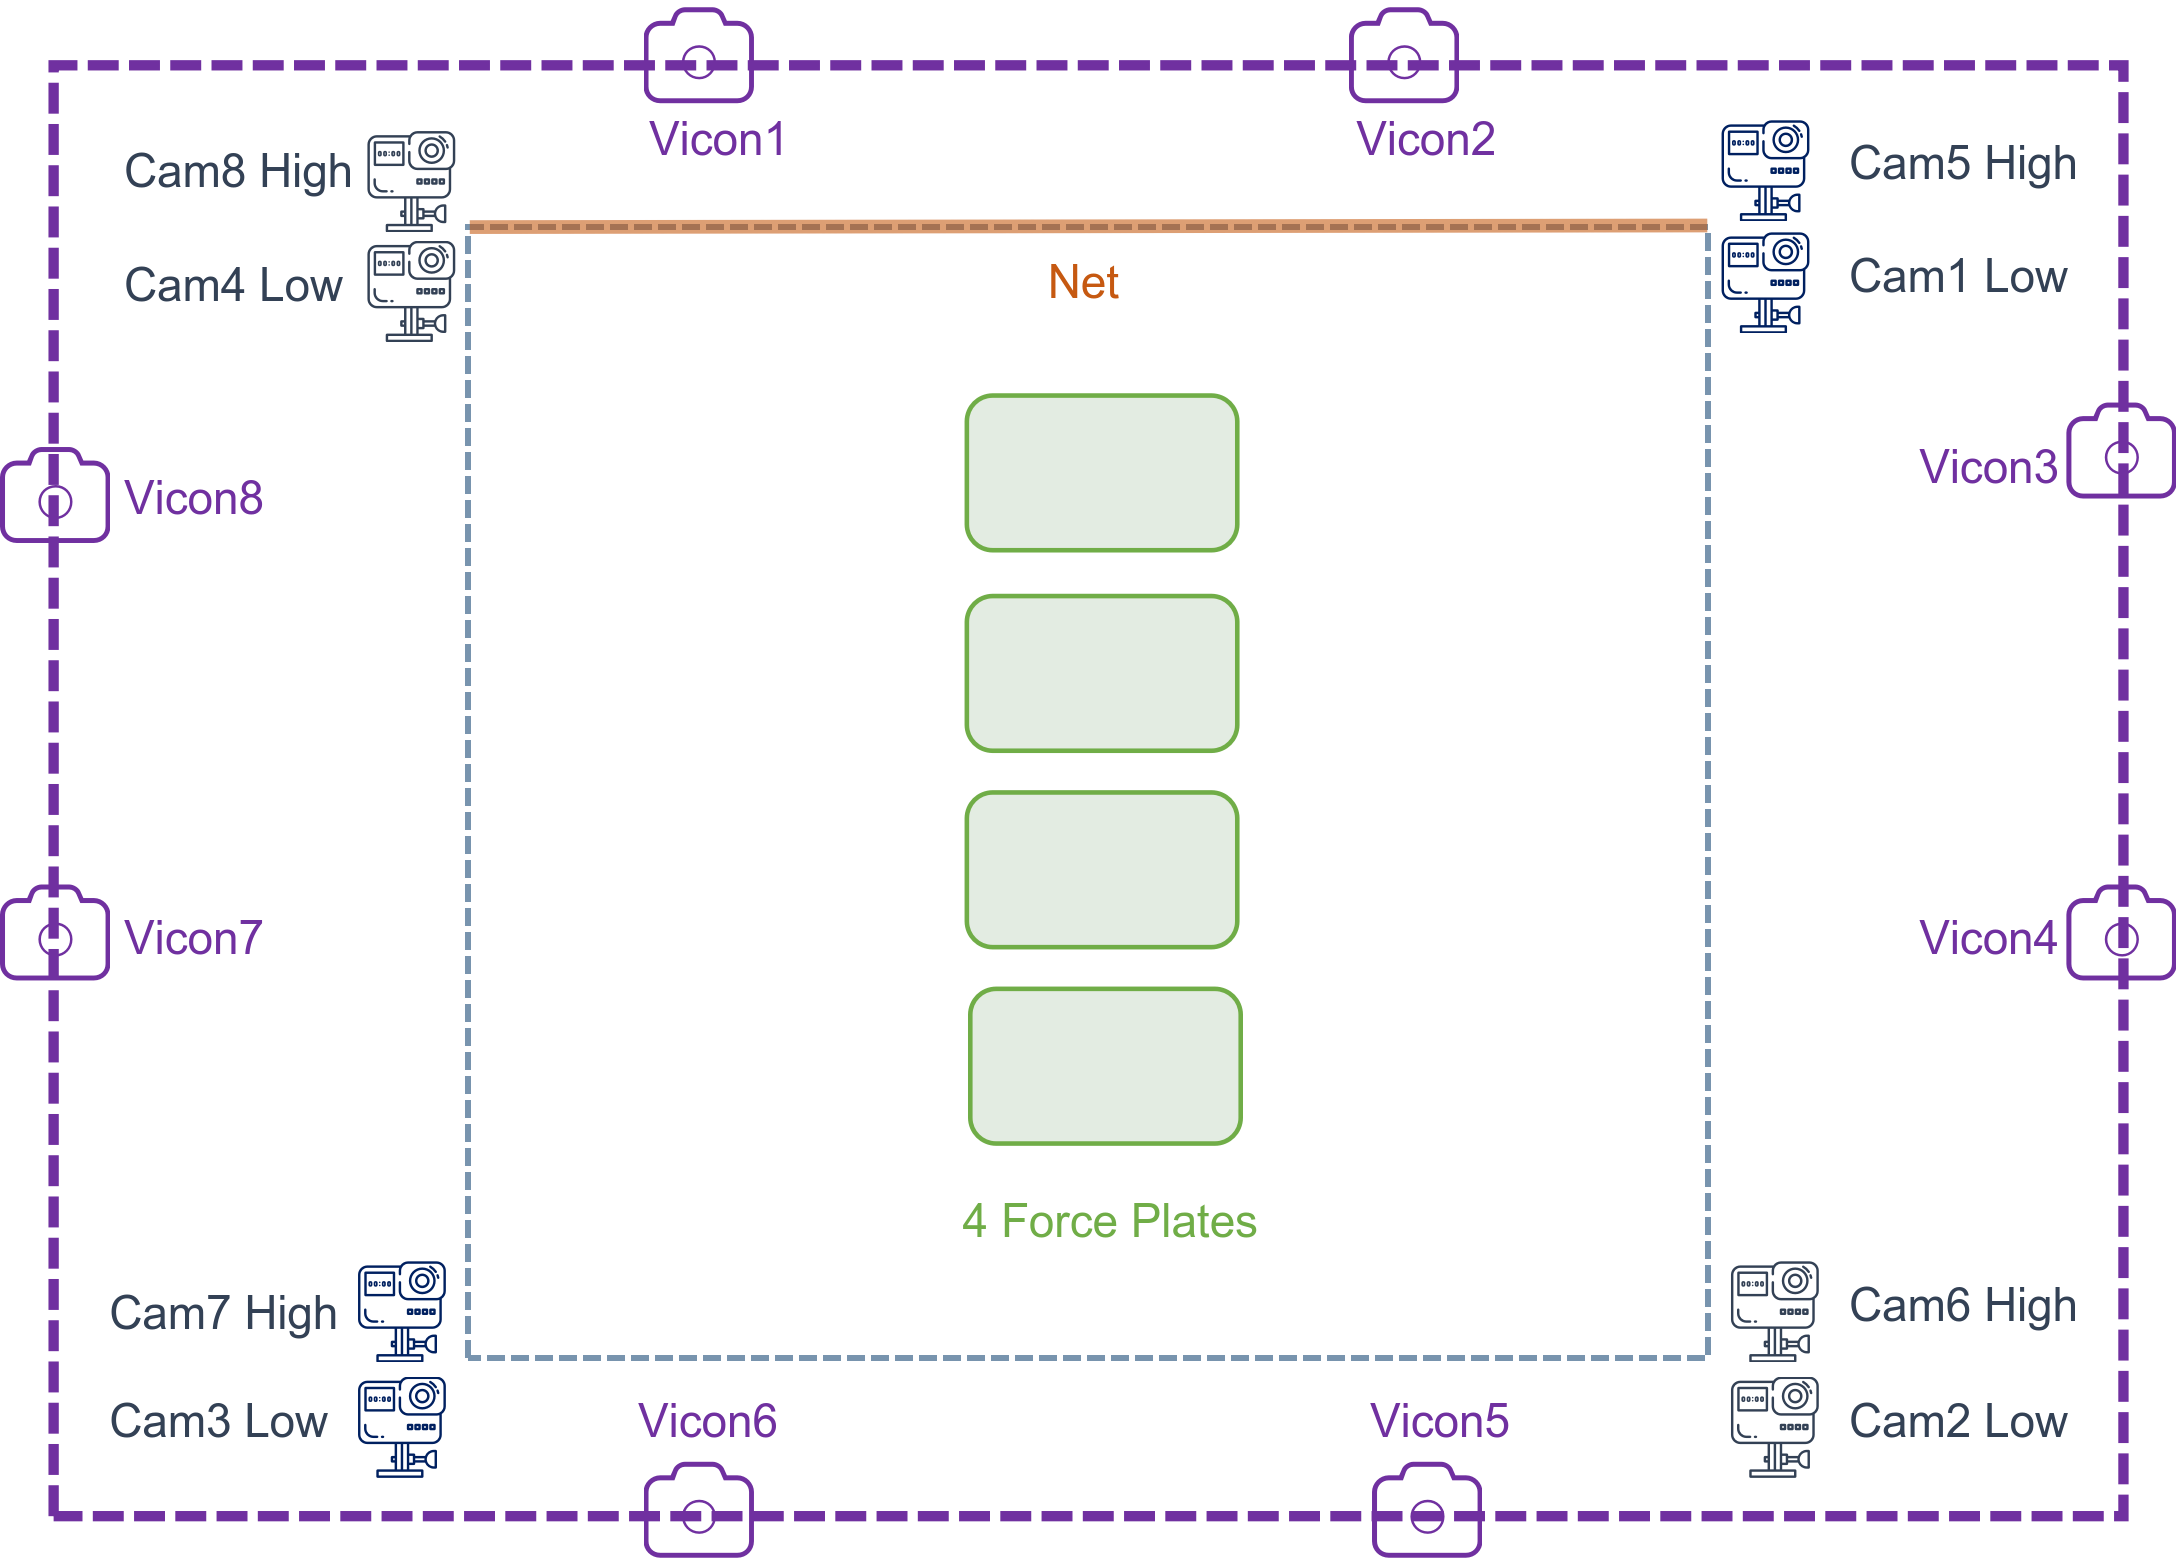
\includegraphics[width=0.86\linewidth]{figures/Fig3.png}%
  \caption{Instrumented acquisition \emph{geometry} (plan view, not to scale): four Kistler plates, eight fixed RGB viewpoints (independent streams), and Vicon motion-capture context. This figure communicates \emph{spatial} sensing layout only; video--GRF time alignment is performed in software after capture (Sec.~\ref{sec:sync_grf}).}
  \label{fig:setup}
  \Description{Plan-view schematic of the instrumented court: force-plate placement, fixed multi-view camera layout, and mocap coverage (not timing).}
\end{figure}

\subsection{Subjects and Protocols}
We collected data from 17 elite badminton athletes (national second-tier and above; IDs: sub\_001--sub\_017). Recruiting such athletes is highly costly due to strict skill, availability, and fatigue-protocol constraints. For the public benchmark release, we report results on 10 subjects (sub\_001--sub\_010) with prepared LOSO splits.
All participants completed structured drills and match-like rallies under both non-fatigue and post-fatigue conditions, with trial tags preserved for downstream stratification \cite{tannion2023Mental,valldecabresEffectMatchFatigue2022,tongEffectsAnkleDorsiflexor2023,gaoAutomatedRecognitionAsymmetric2023,marchena-rodriguezIncidenceInjuriesAmateur2020}. The protocol includes rally plus three footwork stages (upper-net, smash-oriented, six-point reaction), repeated after a full-court fatigue induction.
This protocol design ensures that the released benchmark spans both regular technical drills and workload-shifted conditions.

\subsection{Synchronization and Ground Truth GRF}
\label{sec:sync_grf}
\noindent\textbf{Relation to Fig.~\ref{fig:pipeline}.} Stage~B groups C3D-based GRF export, human-in-the-loop video--GRF alignment, and automatic synchronization \QAabbrev{} checks; Stage~C (pose and tracking) is detailed below.

\paragraph{Heterogeneous clocks and alignment scope.}
Vicon and plates share a laboratory clock; RGB is independently clocked (no genlock). Hardware genlock between consumer cameras and lab systems is rarely available and prohibitively expensive for most research setups, so we use a custom human-in-the-loop alignment UI instead. Annotators mark GRF--video events in this UI; per-camera offsets (about one-frame precision) and uncertainty ship in metadata. Offset uncertainty is derived from frame-level UI annotation tolerance and stored per camera/trial. Residual error is bounded by this procedure and by \(\pm0.5\) s windows (see \BadmintonGRFSupplementary{} for interpolation).

\paragraph{Ground-truth GRF and video--GRF alignment.}
We extract GRF from C3D; four plates sum to a lab-frame wrench; supervision uses contact-positive \(F_z\). The benchmark target is vertical force only (not full multi-axis force regression). Mixed mocap/force rates (\rateHz{240/250}, \rateHz{1000/1200}) are handled in seconds without hard-coded rates.

\paragraph{Synchronization \QAabbrev{}, pose, and tracking (Stage~C).}
Automatic \QAabbrev{} validates offsets; 156 trials, 1,247 $(\text{trial},\text{camera})$ offsets; 65 (5.2\%) flagged for review. QC plots: \BadmintonGRFSupplementary.
\emph{Stage~C}: YOLO26-pose + ByteTrack \cite{chakrabarty2026YOLO26,zhangByteTrackMultiobjectTracking2022}; GRF contact anchors identity across multi-person video.

\begin{table}[t]
  \centering
  \small
  \setlength{\tabcolsep}{4pt}
  \renewcommand{\arraystretch}{1.05}
  \caption{Mini-table: temporal-offset \emph{stress test} on released segments (self-consistency check, not leaderboard metrics; $n=17{,}425$).}
  \label{tab:sync_sensitivity}
  \begin{tabular}{@{}rcccc@{}}
    \toprule
    $\Delta$ frame & $r^2\uparrow$ & RMSE (BW)$\downarrow$ & Peak err (BW)$\downarrow$ & Timing err (fr)$\downarrow$ \\
    \midrule
    $\pm 0$ & 1.000 & 0.000 & 0.000 & 0.00 \\
    $\pm 1$ & 0.951 & 0.133 & 0.534 & 1.03 \\
    $\pm 2$ & 0.869 & 0.220 & 0.923 & 2.03 \\
    $\pm 3$ & 0.779 & 0.286 & 1.094 & 3.02 \\
    \bottomrule
  \end{tabular}
\end{table}
\noindent\emph{Interpretation.} Under synthetic timing jitter, error grows monotonically from $\pm1$ to $\pm3$ frames, supporting our one-frame-level manual alignment target while making the residual timing sensitivity explicit.

\subsection{Segment Construction and Data Statistics}
\label{sec:dataset_stats}
\paragraph{Impact segments and benchmark loader.}
Impact-centric windows and released segment statistics (Fig.~\ref{fig:pipeline}, Stage~D) are summarized below; we detect landing peaks in aligned GRF and extract fixed windows of \(\pm 0.5\) seconds (\(T \approx 120\) frames).
Each benchmark instance is one \emph{impact segment} exported per \((\text{trial},\text{camera},\text{peak})\), with aligned pose/GRF arrays and metadata; full schema and loader contracts are in \BadmintonGRFSupplementary{} and on the \BadmintonGRFRepoShort.
The released benchmark loader applies deterministic quality filters (lower-body mean pose score $<0.70$; tracking lost rate $>0.05$; peak normalized vertical force $>3.0$) and numeric stabilization (low-confidence masking at scores $<0.1$, finite-value sanitation, and bounded clipping for positions/derivatives).

\iffalse
Each impact segment is stored as a NumPy \texttt{.npz} file and corresponds to a fixed window of length
\(T=\lfloor(0.5+0.5)\cdot \texttt{video\_fps}\rceil\) frames around an automatically detected GRF peak.
All arrays use the ordering of time within the segment (index \(i=0,\dots,T-1\)).

\begin{table}[t]
  \centering
  \small
  \setlength{\tabcolsep}{3pt}
  \renewcommand{\arraystretch}{1.05}
  \caption{Impact-segment NPZ keys in \texttt{np.savez} order (exporter: \texttt{pipeline/step4\_segment.py}).}
  \label{tab:segment_schema}
  \begin{tabularx}{\columnwidth}{@{}lX@{}}
    \toprule
    \textbf{Field} & \textbf{Definition} \\
    \midrule
    \texttt{keypoints\_norm} & \((T,17,2)\), float32; \(\texttt{keypoints\_px}/[\texttt{image\_width},\texttt{image\_height}]\), roughly \([0,1]\). \\
    \texttt{keypoints\_px} & \((T,17,2)\), float32; raw COCO-17 \((x,y)\) in pixels. \\
    \texttt{scores} & \((T,17)\), float32; per-joint pose confidence. \\
    \texttt{frame\_indices} & \((T,)\), int32; absolute video frame indices. \\
    \texttt{track\_status} & \((T,)\), NumPy \texttt{U20}; per-frame tracking state (e.g., tracked/pos\_fallback/reidentified/lost). \\
    \texttt{grf\_at\_video\_fps} & \((T,3)\), float32; \([\texttt{Fx},\texttt{Fy},\texttt{Fz}]\) (N), contact-positive \texttt{Fz}>0. \\
    \texttt{grf\_normalized} & \((T,3)\), float32; \(\texttt{grf\_at\_video\_fps}/\max(\texttt{body\_weight\_N},1)\). \\
    \texttt{grf\_1200hz} & \((M,7)\), float32; high-rate window \([\texttt{Fx},\texttt{Fy},\texttt{Fz},\texttt{Fz1},\texttt{Fz2},\texttt{Fz3},\texttt{Fz4}]\) (key name fixed; rate in \texttt{grf\_rate}). \\
    \texttt{timestamps\_video} & \((T,)\), float32; seconds on video axis: \(t_{\text{video}}=\texttt{video\_event\_sec}+(f-\texttt{event\_frame\_abs})/\texttt{video\_fps}\). \\
    \texttt{timestamps\_grf} & \((M,)\), float32; seconds on GRF axis for the \texttt{grf\_1200hz} window. \\
    \texttt{ev\_idx} & int32; peak index within the segment (equals pre-window frame count / \texttt{pre\_frames}). \\
    \texttt{trial} & NumPy str; trial id (includes subject and protocol tags). \\
    \texttt{subject} & NumPy str; \texttt{sub\_XXX} parsed from \texttt{trial}. \\
    \texttt{stage} & NumPy str; protocol stage tag parsed from \texttt{trial}. \\
    \texttt{camera} & int32; camera id \(N\) in \texttt{\_camN\_}. \\
    \texttt{quality} & NumPy str; \texttt{sync.json} alignment quality flag. \\
    \texttt{video\_fps} & float32; effective video frame rate for this clip. \\
    \texttt{grf\_rate} & float32; force-plate nominal sample rate (Hz) read from trial GRF metadata. \\
    \texttt{offset\_sec} & float32; video--GRF time offset (s): \(t_{\text{grf}}=t_{\text{video}}+\texttt{offset\_sec}\). \\
    \texttt{offset\_uncertainty\_sec} & float32; optional uncertainty on \texttt{offset\_sec} from alignment UI. \\
    \texttt{image\_width}, \texttt{image\_height} & int32; frame size used for normalization. \\
    \texttt{body\_weight\_N} & float32; estimated body weight (N) from quiet standing \(F_z\). \\
    \texttt{body\_weight\_kg} & float32; \(\texttt{body\_weight\_N}/9.81\). \\
    \texttt{peak\_force\_N} & float32; \(\max F_z\) over the segment window (N). \\
    \texttt{peak\_force\_bw} & float32; \(\texttt{peak\_force\_N}/\max(\texttt{body\_weight\_N},1)\). \\
    \texttt{impact\_idx} & int32; impact ordinal within this trial/camera (time-sorted). \\
    \texttt{n\_impacts\_total} & int32; total impacts detected for this trial/camera. \\
    \texttt{is\_sync\_impact} & bool; true if this window is anchored at the \texttt{sync.json} alignment event. \\
    \texttt{grf\_peak\_sec} & float32; absolute GRF time (s) of the detected peak. \\
    \texttt{grf\_peak\_N\_detected} & float32; \(F_z\) value (N) at the detected peak before windowing. \\
    \texttt{stat\_lower\_body\_mean\_score} & float32; mean pose score on COCO-17 lower-body joints (11--16). \\
    \texttt{stat\_lost\_rate} & float32; fraction of frames with \texttt{track\_status==lost}. \\
    \texttt{schema\_version} & NumPy str; release-format version tag (see repository). \\
    \texttt{grf\_columns\_hf} & NumPy str; documents \texttt{grf\_1200hz} channel order. \\
    \texttt{grf\_columns\_fps} & NumPy str; documents \texttt{grf\_at\_video\_fps} channel order. \\
    \bottomrule
  \end{tabularx}
\end{table}

\paragraph{Keypoint normalization.}
For each segment we store both \texttt{keypoints\_px} and \texttt{keypoints\_norm}.
Let the pose window provide image size \((W,H)=(\texttt{image\_width},\texttt{image\_height})\).
Then \(\texttt{keypoints\_norm}[i,j,:]=\texttt{keypoints\_px}[i,j,:]/[W,H]\) for frame index \(i\) and joint index \(j\in\{1,\dots,17\}\).

\paragraph{GRF sign convention and units.}
GRF signals are stored in Newton (N).
During GRF loading, the vertical force is converted to a contact-positive convention so that \texttt{grf\_at\_video\_fps} uses \texttt{Fz}>0 for contact.
Horizontal forces \texttt{Fx}/\texttt{Fy} are stored with their native plate coordinate signs (after the same sign harmonization used during GRF extraction).

\paragraph{GRF-to-video alignment (exact interpolation rule).}
Given a segment's video frames with absolute indices \(\{f_i\}\), and the synchronization parameters from \texttt{sync.json}
(\texttt{video\_event\_sec}, \texttt{event\_frame\_abs}, \texttt{video\_fps}, \texttt{offset\_sec}),
the GRF query times are computed as:
\[
 t_{\text{video}}(i)=\texttt{video\_event\_sec} + (f_i-\texttt{event\_frame\_abs})/\texttt{video\_fps},
 \qquad
 t_{\text{grf}}(i)=t_{\text{video}}(i)+\texttt{offset\_sec}.
 \]
For each signal dimension \(\texttt{Fx},\texttt{Fy},\texttt{Fz}\), we linearly interpolate onto \(\{t_{\text{grf}}(i)\}\) using NumPy's
\texttt{np.interp} with constant endpoint extension:
values outside the original GRF timestamp range are clamped to the boundary values.
The resulting interpolated vectors are stored as \texttt{grf\_at\_video\_fps}; \texttt{timestamps\_video} stores \(t_{\text{video}}(i)\) and \texttt{timestamps\_grf} stores the GRF-axis timestamps for the high-frequency window.

\paragraph{High-frequency window \texttt{grf\_1200hz}.}
We additionally store the original GRF samples in a window centered at the detected peak time:
\[
 t\in[\texttt{grf\_peak\_sec}-0.5,\ \texttt{grf\_peak\_sec}+0.5].
 \]
Let \(M\) be the number of GRF samples satisfying the mask; then \texttt{grf\_1200hz} has shape \((M,7)\) and \texttt{timestamps\_grf} has shape \((M,)\).

\paragraph{Segment generation skip rules (peak detection and window feasibility).}
Before saving a segment, our segmentation pipeline enforces:
(i) \texttt{sync.json} quality must be in \{\texttt{"good"}, \texttt{"ok"}, empty\}; otherwise the (trial,cam) is skipped.
(ii) Candidate landing peaks are detected on GRF vertical force after a 4th-order Butterworth low-pass filter (cutoff 50~Hz, used only for detection).
We run \texttt{find\_peaks} with thresholds in body-weight units:
\( \texttt{height} \ge 0.5\times \texttt{body\_weight\_N}\),
\( \texttt{prominence} \ge 0.2\times \texttt{body\_weight\_N}\),
and a minimum peak distance of 250~ms.
(iii) Each detected peak is mapped to the nearest pose frame using \texttt{frame\_indices}; peaks are discarded if a \(\pm 0.5\)s window cannot be fully covered by available pose frames.
(iv) Overlapping detections are deduplicated by keeping the larger peak when their mapped pose indices overlap the full window.
If no valid peaks are found, the pipeline falls back to a single impact at the synchronization event frame, provided the window is feasible.

\paragraph{Loader-level segment filtering (exact thresholds used by the benchmark).}
When building training/test datasets, we load all released impact-segment \texttt{.npz} files but discard invalid segments using the following thresholds (as specified for the released benchmark loader):
discard a segment if any of the conditions holds:
\[
\texttt{stat\_lower\_body\_mean\_score} < 0.70
\ \ \text{or}\ \ 
\texttt{stat\_lost\_rate} > 0.05
\ \ \text{or}\ \ 
\texttt{peak\_force\_bw} > 3.0.
\]
This ensures that the released benchmark mainly contains windows with reliable lower-body pose and limited tracking failures, while excluding outlier impacts with unusually large forces.

\paragraph{Loader numeric handling (NaNs and low-confidence masking).}
The benchmark input features are built from \texttt{keypoints\_norm} and \texttt{scores} by applying deterministic numeric rules:
(i) frames with \(\texttt{scores}<0.1\) are treated as invalid, and their keypoint coordinates are set to zero;
(ii) remaining \texttt{keypoints\_norm} values are sanitized with \texttt{nan\_to\_num} (NaN/Inf replaced by finite values), and then position coordinates are clipped to \([0,1]\);
(iii) velocities and accelerations are computed as first and second forward differences, with their outputs also clipped to \([-0.5,0.5]\) to avoid exploding gradients or NaN propagation.

This design supports direct learning from pose sequences while preserving alignment provenance; we refer to the stored representation as the BadmintonGRF segment representation in the rest of the paper.

\fi
\paragraph{Dataset statistics.}
Tier~1 contains 17{,}425 archives. After loader gates, 12{,}867 instances remain, corresponding to 1{,}732 unique impacts (deduplicated). The release includes 156 trials. About \(\sim\)7\% windows use sync-event fallback (metadata flag, not sync failure). Stage-stratified stats and $N\!\in\![5,10]$ LOSO bundles are provided in \BadmintonGRFSupplementary{} and on the \BadmintonGRFRepoShort. Table~\ref{tab:stats} summarizes scope.

\begin{table}[t]
  \centering
  \small
  \setlength{\tabcolsep}{4pt}
  \renewcommand{\arraystretch}{1.05}
  \caption{Mini-table: loader-gate audit on released segments (from in-repo reports).}
  \label{tab:filter_audit}
  \begin{tabular}{@{}lccc@{}}
    \toprule
    Split & Segments & Unique impacts & Mean $|\mathrm{lag}_{F_z,CoM_y}|$ (fr) \\
    \midrule
    Before gates & 17{,}425 & 2{,}263 & 15.89 \\
    After gates & 12{,}867 & 1{,}732 & 15.71 \\
    \bottomrule
  \end{tabular}
\end{table}
\noindent Table~\ref{tab:filter_audit} summarizes the effect of quality gates. \emph{Distribution shift check.} Retention is 73.8\%; maximum stage-share shift is 13.05 percentage points and maximum subject-share shift is 2.21 points after gating, indicating stronger stage-wise than subject-wise selection effects.

\begin{table}[t]
  \centering
  \small
  \setlength{\tabcolsep}{4pt}
  \renewcommand{\arraystretch}{1.05}
  \caption{Released benchmark scope: 10-subject LOSO subset and acquisition statistics (processed segments and metadata).}
  \label{tab:stats}
  \begin{tabularx}{\columnwidth}{@{}lX@{}}
    \toprule
    \textbf{Item} & \textbf{Value} \\
    \midrule
    Subjects (benchmark) & 10 (sub\_001--sub\_010) \\
    Subjects (collected) & 17 (complete; ongoing collection) \\
    Cameras & 8 DJI Osmo Action 4, 1080p, \(\sim\)120 FPS \\
    Force plates & 4 Kistler 9260AA6 plates, 6-axis GRF \\
    Force sampling rate & \rateHz{1000/1200} (\(=4\!\times\)\rateHz{250/240} mocap; per-trial metadata) \\
    Mocap & 8 Vicon T40 cameras, \(\sim\)52-marker protocol (14 mm; session counts vary slightly), C3D (raw markers preserved) \\
    Mocap sampling rate & \rateHz{240/250} (\(=1/4\) force rate; per-trial metadata) \\
    Impact segments & 17{,}425 archived segments; 12{,}867 after quality gates; 1{,}732 unique impacts (post-gate multi-view dedup.); 156 trials \\
    Segment window & \(\pm 0.5\) s, \(T\approx 120\) frames \\
    \bottomrule
  \end{tabularx}
\end{table}

\subsection{Data Access and Privacy}
Tier~1 provides processed pose, GRF, metadata, and splits (public).
The dataset is available at Zenodo: \url{https://doi.org/10.5281/zenodo.19277566}.
Tier~2 provides raw RGB + C3D under application access, with no redistribution and no re-identification.
Extended schema, loader specifications, and DOI/access workflow are documented in \BadmintonGRFSupplementary{} and on the \BadmintonGRFRepoShort.

%================ 4--5. Benchmark and Evaluation (Dataset Track) ================
\section{Benchmark and Evaluation}
\label{sec:benchmark_methods}
\label{sec:experiments}
\noindent We evaluate \emph{resource utility} (Fig.~\ref{fig:pipeline}, Stage~E): baselines are reproducible anchors, not a leaderboard. Read Table~\ref{tab:benchmark_all} by \textsc{LOSO} SV \(r^2\) (cross-subject), then \textsc{LOSO} Fus (fusion trade-offs), then Within (weaker shift). All ten models share LOSO splits, 15\% val per fold, best-val checkpoint, single test forward pass (no TTA); defaults in \BadmintonGRFSupplementary{}.

\begin{table*}[!t]
  \centering
  \footnotesize
  \setlength{\tabcolsep}{2.4pt}
  \renewcommand{\arraystretch}{1.12}
  \caption{\textbf{Benchmark} (macro means over folds; \(\uparrow\) better \(r^2\); \(\downarrow\) better \textbf{R}/\textbf{P}/\textbf{T}). \textbf{\textsc{LOSO} SV/Fus}: leave-one-subject-out \(\pm\) late fusion. \textbf{Within}: within-trial. \textbf{R}: RMSE \(F_z\) (BW); \textbf{P}: peak error (BW); \textbf{T}: peak timing (frames). Bold: best per block. Fold std: \BadmintonGRFSupplementary.}
  \label{tab:benchmark_all}
  \resizebox{\textwidth}{!}{%
  \begin{tabular}{@{}l cccc cccc cccc cccc@{}}
    \toprule
    & \multicolumn{4}{c}{\textbf{\textsc{LOSO} SV}} & \multicolumn{4}{c}{\textbf{\textsc{LOSO} Fus}} & \multicolumn{4}{c}{\textbf{Within SV}} & \multicolumn{4}{c}{\textbf{Within Fus}} \\
    \cmidrule(lr){2-5} \cmidrule(lr){6-9} \cmidrule(lr){10-13} \cmidrule(lr){14-17}
    \textbf{Model} & \(r^2\,\uparrow\) & \textbf{R}\,\(\downarrow\) & \textbf{P}\,\(\downarrow\) & \textbf{T}\,\(\downarrow\) & \(r^2\,\uparrow\) & \textbf{R}\,\(\downarrow\) & \textbf{P}\,\(\downarrow\) & \textbf{T}\,\(\downarrow\) & \(r^2\,\uparrow\) & \textbf{R}\,\(\downarrow\) & \textbf{P}\,\(\downarrow\) & \textbf{T}\,\(\downarrow\) & \(r^2\,\uparrow\) & \textbf{R}\,\(\downarrow\) & \textbf{P}\,\(\downarrow\) & \textbf{T}\,\(\downarrow\) \\
    \midrule
    PatchTST~\cite{nieTimeSeriesWorth2023}                     & \textbf{0.403} & \textbf{0.510} & 0.226 & 1.07 & 0.412 & 0.584 & 0.693 & 1.48 & 0.494 & 0.470 & 0.211 & 1.33 & 0.304 & 0.634 & 0.719 & 3.98 \\
    ST-GCN+Transformer~\cite{shiSkeletonBasedActionRecognition2019,shiTwoStreamAdaptiveGraph2019,vaswaniAttention2017}           & 0.394 & 0.514 & 0.221 & \textbf{0.96} & 0.454 & \textbf{0.487} & \textbf{0.210} & \textbf{0.90} & 0.576 & 0.430 & \textbf{0.191} & \textbf{1.27} & \textbf{0.617} & \textbf{0.408} & \textbf{0.182} & \textbf{1.15} \\
    TCN+BiGRU~\cite{baiEmpiricalEvaluationConvolutional2018,choLearningPhraseRepresentations2014}                    & 0.390 & 0.514 & 0.348 & 3.79 & 0.274 & 0.645 & 0.952 & 6.51 & 0.519 & 0.456 & 0.407 & 4.27 & 0.167 & 0.690 & 1.025 & 8.99 \\
    TCN+BiLSTM~\cite{baiEmpiricalEvaluationConvolutional2018,hochreiterLongShortTermMemory1997}                   & 0.374 & 0.521 & 0.309 & 2.58 & 0.370 & 0.602 & 0.960 & 3.73 & 0.547 & 0.443 & 0.365 & 3.96 & 0.151 & 0.696 & 1.021 & 8.93 \\
    TSMixer~\cite{chenTSMixerAllMLP2023}                      & 0.351 & 0.531 & \textbf{0.218} & 1.85 & \textbf{0.472} & 0.553 & 0.673 & 1.22 & \textbf{0.635} & \textbf{0.395} & 0.201 & 1.67 & 0.414 & 0.579 & 0.645 & 2.11 \\
    Seq-Transformer~\cite{vaswaniAttention2017}              & 0.345 & 0.533 & 0.281 & 1.82 & 0.336 & 0.619 & 0.870 & 2.37 & 0.517 & 0.458 & 0.245 & 1.69 & 0.032 & 0.745 & 0.900 & 5.36 \\
    PatchTST-XL~\cite{nieTimeSeriesWorth2023}                  & 0.339 & 0.535 & 0.224 & 1.46 & 0.456 & 0.561 & 0.656 & 1.38 & 0.597 & 0.417 & 0.216 & 1.45 & 0.374 & 0.600 & 0.713 & 2.58 \\
    TCN+MLP~\cite{baiEmpiricalEvaluationConvolutional2018}                      & 0.275 & 0.562 & 0.432 & 9.29 & 0.327 & 0.625 & 1.103 & 9.47 & 0.341 & 0.537 & 0.587 & 12.68 & 0.107 & 0.716 & 1.055 & 13.89 \\
    MS-TCN~\cite{farhaMSTCN2019}                       & 0.184 & 0.596 & 0.688 & 14.24 & 0.232 & 0.667 & 1.313 & 13.92 & 0.122 & 0.621 & 0.764 & 15.34 & 0.135 & 0.708 & 1.357 & 15.11 \\
    DLinear~\cite{zengAreTransformersEffective2023}                      & 0.072 & 0.636 & 0.819 & 16.03 & 0.149 & 0.702 & 1.432 & 15.11 & 0.003 & 0.662 & 0.939 & 15.96 & 0.021 & 0.753 & 1.532 & 15.09 \\
    \bottomrule
  \end{tabular}%
  }
  \vspace{2pt}
  {\scriptsize\setlength{\baselineskip}{10.4pt}%
  \noindent\emph{Reproducibility:} archived runs; bundle ids in \BadmintonGRFSupplementary{}.}
\end{table*}

\noindent\textbf{Task and models.}
Tier~1 uses a \textbf{keypoint-first} task: regress BW-\(F_z\) from COCO-17 pose and confidences (plus velocities/accelerations) \cite{mundt2022Estimating,ishida2024Estimation,hossain2025Knowledge}, conditioned on aligned impacts (Sec.~\ref{sec:dataset_stats}).
We benchmark ten architectures: TCN+BiLSTM, TCN+BiGRU, TCN+MLP, Transformer, DLinear, PatchTST, PatchTST-XL, MS-TCN, TSMixer, and ST-GCN+Transformer \cite{baiEmpiricalEvaluationConvolutional2018,hochreiterLongShortTermMemory1997,choLearningPhraseRepresentations2014,vaswaniAttention2017,zengAreTransformersEffective2023,nieTimeSeriesWorth2023,chenTSMixerAllMLP2023,farhaMSTCN2019,shiSkeletonBasedActionRecognition2019,shiTwoStreamAdaptiveGraph2019}.

\paragraph{LOSO, fusion, and within-trial.}
LOSO on 10 subjects; 15\% val; metrics macro-averaged: \(r^2\), RMSE \(F_z\) (BW), peak error, peak timing (frames) \cite{ishida2024Estimation,mundt2022Estimating}. Late fusion post-hoc (confidence weights) can raise \(r^2\) while hurting RMSE---report all four metrics. Within-trial: held-out impacts in the same trials (upper-bound diagnostic). Scaling $N\!\in\![5,10]$, ablations, \QAabbrev{} plots: \BadmintonGRFSupplementary.

\paragraph{Reading Table~\ref{tab:benchmark_all}.}
We use a three-level interpretation hierarchy. \textbf{Level-1 (primary)} is LOSO single-view, which best reflects cross-subject generalization; PatchTST and ST-GCN+Transformer are strongest here. \textbf{Level-2 (systems gain)} is LOSO with late fusion, where \(r^2\) often improves but RMSE/peak error may not, so all four metrics must be read jointly. \textbf{Level-3 (diagnostic upper bound)} is within-trial, which is intentionally easier and should not be treated as a deployment proxy. Table~\ref{tab:benchmark_all} pools rally/stage/fatigue tags; stratified diagnostics are in \BadmintonGRFSupplementary.

\noindent\textbf{Applications and artifact release.}
Beyond benchmarking, the resource supports training-load analytics, fatigue-stratified studies, and occlusion-aware multi-view learning \cite{johnsonOnfieldPlayerWorkload2019,gaoAutomatedRecognitionAsymmetric2023,mundt2022Estimating,bogaertPredictingVerticalGround2024}. Tier~1 pose+GRF and documentation are released under CC BY-NC~4.0; code is released under MIT; raw RGB/C3D follow Tier~2 controlled-access terms on the \BadmintonGRFRepoShort. Step-by-step reproduction aligns with reporting guidance \cite{hebert-losierReportingGuidelinesRunning2023}.

\subsection{Reproducibility and Benchmark Protocol Notes}
\label{sec:repro_notes}
To make BadmintonGRF immediately reusable as a \emph{dataset track} artifact, we package not only data files but also protocol-level decisions that are often implicit in prior pose-to-force work.
In practice, two groups can report the same model family yet obtain noticeably different values if they differ in fold construction, quality filtering, or post-processing.
For this reason, each released run bundle includes: subject-level split manifests, deterministic segment lists after loader gates, random seeds, optimizer and scheduler defaults, and a metric script that recomputes all four headline metrics from raw predictions.
This design separates dataset effects from implementation variance and improves comparability across independent reproductions.
For transparency, the artifacts behind Tables~\ref{tab:sync_sensitivity} and~\ref{tab:filter_audit} are released on the project repository as a versioned supplementary audit bundle (machine-readable JSON plus human-readable markdown).

\paragraph{Artifact checklist (main-paper index).}
The release includes five items: (i) subject-level LOSO split manifests; (ii) deterministic segment lists after loader gates; (iii) training/evaluation command templates; (iv) canonical metric keys and table-export scripts; and (v) synchronization and filter-audit artifacts used by this manuscript.
Detailed commands and file-level schema remain in \BadmintonGRFSupplementary{} and the repository documentation.

\paragraph{Protocol hierarchy for fair comparison.}
We recommend reading benchmark outcomes in a three-level hierarchy.
Level~1 is \textsc{LOSO} single-view, which best reflects cross-subject transfer under minimal assumptions.
Level~2 adds post-hoc multi-view late fusion and should be interpreted as a \emph{systems} gain that depends on camera availability and confidence calibration.
Level~3 is within-trial evaluation, which is intentionally easier and should be treated as a diagnostic upper bound rather than a deployment proxy.
Under this hierarchy, a method should first demonstrate stable \textsc{LOSO} behavior before within-trial gains are considered practically meaningful.

\paragraph{Metric trade-offs.}
Impact-centric force traces have narrow high-curvature regions around landing peaks.
Therefore, scalar summary metrics are coupled in non-trivial ways.
For example, a smoother predictor may reduce RMSE while increasing peak attenuation, and a sharper predictor may improve peak magnitude while slightly worsening timing jitter.
Therefore, we recommend reporting all four metrics jointly and avoiding single-number ranking claims.
In coaching-facing applications, the preferred operating point may differ by use case: workload trend monitoring often prioritizes RMSE stability over many impacts, whereas return-to-play screening may prioritize peak and timing fidelity for high-load events.
The released scripts support this multi-objective reading by exporting per-impact residuals in addition to fold-level aggregates.

\paragraph{Generalization diagnostics enabled by metadata.}
A practical advantage of BadmintonGRF is that stage and fatigue annotations are native to the trial identity.
This allows users to test whether a model trained on mixed data exhibits systematic degradation in specific protocol stages (e.g., six-point reaction under post-fatigue conditions).
Such stratified evaluation is crucial when transferring models from laboratory-style benchmarks to real training contexts, where distribution shift is driven more by task intensity and athlete state than by camera viewpoint alone.
To facilitate this analysis, we release stage/fatigue index files and script hooks for grouped metric aggregation without modifying core loaders.

\paragraph{Recommended reporting checklist.}
For transparent comparisons, we suggest reporting at least the following items with each experiment: (i) subject IDs in train/val/test for every fold; (ii) number of retained segments and unique impacts after quality gates; (iii) whether confidence masking and derivative clipping are enabled; (iv) whether fusion weights are fixed globally or tuned per fold; (v) fold-wise mean and standard deviation for all four metrics.
This checklist is lightweight to adopt and directly addresses common reproducibility gaps in multimodal biomechanical benchmarks.

%================ (Practicalities merged into Discussion) ================

%================ 7. Discussion and Limitations ================
\section{Discussion and Limitations}
\label{sec:limitations}
Synchronization \QAabbrev{}, protocol metadata, and impact-centric segmentation improve benchmark stability; fixed preprocessing makes model comparisons more interpretable \cite{evansSynchronisedVideoMotion2024,hebert-losierReportingGuidelinesRunning2023}.

\noindent\textbf{Alignment vs.\ genlock.}
Consumer RGB is not clock-locked to laboratory plates; we use human-verified per-camera offsets with automatic \QAabbrev{} and released uncertainty (Sec.~\ref{sec:sync_grf}). Residual error is non-zero but bounded; \(\pm0.5\) s windows support practical tolerance.

\noindent\textbf{Tier~1 vs.\ Tier~2.}
Tier~1 (pose+GRF, metadata, splits) reproduces Table~\ref{tab:benchmark_all} without raw RGB/C3D. Tier~2 enables video/mocap studies under approval; it does not redefine the Tier~1 task.

\noindent\textbf{Validity and coverage.}
The open tree covers ten athletes at one venue; we expect gains as the 17-subject cohort finishes \QAabbrev{} (\(N\!\in\![5,10]\) scaling: \BadmintonGRFSupplementary). Loader gates withhold \(\sim\)26\% of exports for pose/tracking/peak hygiene; \(\sim\)7\% windows anchor at sync events when auto peak detection fails (metadata flag---not sync failure). Heterogeneous camera settings are flagged for analysis.

\noindent\textbf{Ethics.}
Participants gave informed consent for tiered capture (identifiable video under Tier~2 rules). Extended ethics wording and reproduction bundles: \BadmintonGRFSupplementary{}.

\noindent\textbf{Practical reuse guidance.}
To reduce hidden variance across labs, we recommend reporting four implementation choices together with metrics: (i) whether training uses only quality-gated windows or all exports, (ii) whether low-confidence joints are masked before derivative features, (iii) whether late fusion is tuned per fold or fixed globally, and (iv) whether evaluation includes stage/fatigue stratification in addition to macro means.
In pilot replications, these choices changed RMSE and peak metrics even when model architecture was unchanged, indicating that data-handling details are a first-order factor in impact-centric GRF estimation.

\noindent\textbf{Failure modes and future extensions.}
Current errors mainly cluster in three settings: severe lower-body occlusion, abrupt identity switches during crossing trajectories, and rare high-impact outliers near the quality-gate boundary.
The released metadata enables targeted analyses of these regimes and supports straightforward extensions: uncertainty-aware losses using offset uncertainty, stage-conditional evaluation under fatigue tags, and geometry-aware multi-view fusion that exploits fixed camera placement.
As additional subjects complete QA, expanding LOSO to the full cohort will improve statistical power for cross-subject generalization and for subgroup analyses (e.g., stage-specific landing mechanics).

\section{Conclusion}
We presented BadmintonGRF: badminton court trials with laboratory GRF, software alignment without hardware genlock, and a reproducible pose-to-GRF benchmark with ten reference models and late fusion.
Tier~1 enables privacy-preserving replication; Tier~2 supports controlled multimodal extensions. We expect this resource to advance impact-centric load estimation and multimodal sports datasets.

%================ Acknowledgements（可选） ================
% \begin{acks}
% TODO: 致谢与资助信息（若有）。
% \end{acks}

%================ 参考文献 ================
% Dataset Track: keep main text (through Conclusion) within the page budget; references follow.
% ACM \texttt{ACM-Reference-Format}: reference list is ordered alphabetically by author, not by citation order.
\clearpage
\balance
\bibliographystyle{ACM-Reference-Format}
\bibliography{ACM_MM_2026}

\end{document}

